%
%  Peter Vermeer
%
\documentclass[12pt,fullpage]{article}
\usepackage{fullpage}
\usepackage{psfrag}                                          % LaTeX graphics tool
\usepackage{pslatex}                                         % avoids the default cmr font
\usepackage{graphicx}                                        % graphics package 
\usepackage{epsfig}                                          % figures
\usepackage{hyperref}
\usepackage{color}

\begin{document}

\noindent
{\bf Discrete Weibull distribution} (from \color{blue}\url{http://www.math.wm.edu/~leemis/chart/UDR/UDR.html}\color{black})

\noindent
The shorthand $X \sim {\rm Discrete\ Weibull}(p,\, \beta)$ is used to indicate that the
random variable $X$ has the discrete Weibull distribution with real parameter $p$ satisfying $0 < p < 1$, and positive shape parameter $\beta$.
A discrete Weibull random variable $X$ with parameters $p$ and $\beta$ has probability mass function 
$$
f(x) = (1 - p) ^ {x ^ {\kern 0.08 em \beta}} - (1 - p) ^ {(x + 1) ^ {\beta}} \qquad \qquad x=0,1,2,\ldots .
$$
The probability mass function for three different parameter settings is illustrated below.

\begin{figure}[h!]
\begin{center}
\psfrag{labx}{$x$}
\psfrag{labf}{$f(x)$}
\psfrag{labp3}{$p = 0.3$}
\psfrag{labp6}{$p = 0.6$}
\psfrag{labb1}{$\beta = 1$}
\psfrag{labb2}{$\beta = 2$}
\includegraphics[width=5.8in]{DiscreteweibullPlot.ps}
\end{center}
\end{figure}

\noindent
The cumulative distribution function on
the support of $X$ is
$$
F(x) = P(X \le x) = 1 - \left( 1 - p \right) ^ { \left( x + 1 \right) ^ {\mbox {{\tt}}_{{\beta}}}}  \qquad \qquad x=0,1,2,\ldots.
$$
The survivor function on the support of $X$ is
$$
S(x) = P(X \ge x) =  \left( 1 - p \right) ^ { x^ {\beta}}  \qquad \qquad x=0,1,2,\ldots.
$$
The hazard function on the support of $X$ is
$$
h(x) = \frac{f(x)} {S(x)} = 1 - \left( 1 - p \right) ^ {\left( x + 1 \right) ^ {\beta}- x^{\beta}} \qquad \qquad x=0,1,2,\ldots.
$$
The cumulative hazard function on the support of $X$ is
$$
H(x) = - \ln S(x) = -{x} ^ {\kern 0.08 em \beta} \ln  \left( 1 - p \right)  \qquad \qquad x=0,1,2,\ldots.
$$
The inverse distribution function of $X$ is mathematically intractable.

\vspace{0.1in}

\noindent
The moment generating function of $X$ is
$$
M(t) = E\left[ e ^ {\kern 0.08 em tX} \right] = \sum _{x = 0} ^ {\infty } \left( (1-p)^{x^{\beta}} - (1 - p)^{(x+1)^{\beta}} \right) e^{tx}.
$$
The population mean of $X$ is  
$$
E\left[ X \right] = \sum _{x = 0} ^ {\infty } \left( \left( 1 - p \right)  ^ {{x} ^ {\kern 0.08 em \beta}} - \left( 1 - p \right) ^ { \left( x + 1 \right) ^ {\beta}} \right) x.
$$
The variance, skewness, and kurtosis of $X$ are mathematically intractable in the generalized case.

\vspace{0.1in}

\noindent
{\bf APPL verification:}
The APPL statements
\begin{verbatim}
X := [[x->(1-p)^(x^b)-(1-p)^((x+1)^b)], [0 .. infinity], ["Discrete", "PDF"]];
CDF(X);
SF(X);
CHF(X);
MGF(X);
Mean(X);
\end{verbatim}
verify the cumulative distribution function, survivor function, cumulative hazard function, moment generating function, and population mean.

\end{document}
